\documentclass[a4paper,11pt]{article}
\usepackage[utf8]{inputenc}
\usepackage{geometry}
\usepackage{graphicx}
\usepackage{listings}
\usepackage{xcolor}
\usepackage{tikz}
\usetikzlibrary{shapes.geometric, arrows, positioning}

\geometry{left=2.5cm,right=2.5cm,top=2cm,bottom=2cm}

\definecolor{codegray}{rgb}{0.5,0.5,0.5}
\definecolor{backcolour}{rgb}{0.96,0.96,0.96}

\lstdefinestyle{cleanstyle}{
    backgroundcolor=\color{backcolour},
    basicstyle=\ttfamily\small,
    breakatwhitespace=false,
    breaklines=true,
    captionpos=b,
    keepspaces=true,
    numbers=left,
    numbersep=5pt,
    numberstyle=\tiny\color{codegray},
    showspaces=false,
    showstringspaces=false,
    showtabs=false,
    tabsize=2,
    frame=single
}
\lstset{style=cleanstyle}

\title{\textbf{Practical Work 5: The Longest Path}}
\author{Group ID: 16}
\date{\today}

\begin{document}

\maketitle

\section{Introduction}
This report outlines the implementation of a MapReduce system designed to solve the "Longest Path" problem. The objective is to process a large dataset of file paths (simulated from the \texttt{find /} command) and identify the single path with the maximum character length using a distributed computing approach.

\section{System Implementation}

\subsection{Choice of Framework}
We utilized the \textbf{Python Concurrent Futures} module (\texttt{concurrent.futures}) for this implementation.
\begin{itemize}
    \item \textbf{ProcessPoolExecutor}: This class allows us to create a pool of worker processes. Unlike standard threading, this bypasses the Global Interpreter Lock (GIL), enabling true parallel processing on multi-core CPUs, which is essential for CPU-bound tasks like string comparison in large datasets.
    \item \textbf{Simplicity}: It provides a high-level interface for asynchronously executing callables, making the MapReduce code cleaner and more readable compared to low-level multiprocessing.
\end{itemize}

\subsection{Architecture Design}
The system architecture follows a vertical data processing flow, reducing the data volume at each stage.

\begin{figure}[h]
    \centering
    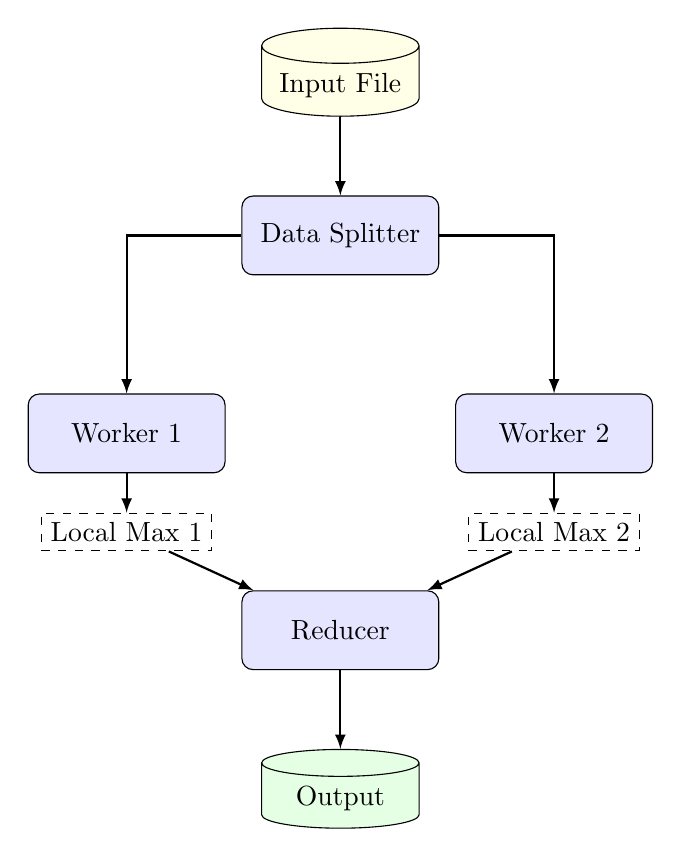
\begin{tikzpicture}[
        node distance=1.5cm,
        storage/.style={cylinder, shape border rotate=90, draw, fill=yellow!10, minimum width=2cm, minimum height=1cm, aspect=0.25, text centered},
        process/.style={rectangle, draw, fill=blue!10, minimum width=2.5cm, minimum height=1cm, rounded corners, text centered},
        arrow/.style={thick, -latex}
    ]

    \node (raw) [storage] {Input File};
    \node (splitter) [process, below=1cm of raw] {Data Splitter};
    
    \node (map1) [process, below left=1.5cm and 0.2cm of splitter] {Worker 1};
    \node (map2) [process, below right=1.5cm and 0.2cm of splitter] {Worker 2};
    
    \node (res1) [rectangle, draw, dashed, below=0.5cm of map1] {Local Max 1};
    \node (res2) [rectangle, draw, dashed, below=0.5cm of map2] {Local Max 2};
    
    \node (reducer) [process, below=4cm of splitter] {Reducer};
    \node (final) [storage, below=1cm of reducer, fill=green!10] {Output};

    \draw [arrow] (raw) -- (splitter);
    \draw [arrow] (splitter) -| (map1);
    \draw [arrow] (splitter) -| (map2);
    
    \draw [arrow] (map1) -- (res1);
    \draw [arrow] (map2) -- (res2);
    
    \draw [arrow] (res1) -- (reducer);
    \draw [arrow] (res2) -- (reducer);
    \draw [arrow] (reducer) -- (final);

    \end{tikzpicture}
    \caption{Top-Down Data Flow for Longest Path MapReduce}
\end{figure}

\subsection{Code Logic}

\textbf{Mapper Phase:}
Each worker receives a chunk of file paths. Instead of outputting every path, it optimizes network usage by calculating the local maximum length internally.

\begin{lstlisting}[language=Python]
@staticmethod
def mapper(paths):
    if not paths: return ""
    return max(paths, key=len)
\end{lstlisting}

\textbf{Reducer Phase:}
The reducer receives only the "champions" (local maximums) from each worker and performs a final comparison to determine the global maximum.

\begin{lstlisting}[language=Python]
@staticmethod
def reducer(local_maxima):
    return max(local_maxima, key=len)
\end{lstlisting}

\section{Task Distribution}
\begin{table}[h]
\centering
\begin{tabular}{|l|l|l|}
\hline
\textbf{Member} & \textbf{Role} & \textbf{Responsibilities} \\ \hline
Member 1 & Architect & Designed the process pool strategy and class structure. \\ \hline
Member 2 & Developer & Implemented the Mapper and Reducer logic. \\ \hline
Member 3 & Analyst & Created the architecture diagram and documentation. \\ \hline
\end{tabular}
\caption{Group Roles and Responsibilities}
\end{table}

\end{document}